\subsection{Cross Compatibility of CPUs}
Whenever customer try to change the default Intel motherboard CPU with different Intel silicon chip which won’t works. The specific CPU Chip initialization varies for each generation. So, the board designs should be designed is such a way that specific generation CPU should support., if we change the CPU with a different Intel Board it will not even boot, because the BIOS doesn't support for other Silicon Initialization for other CPUs.

So, we are integrating the runtime detection of the silicon during the Pre-Extensible Firmware Initialization (\gls{pei}) phase. So, within single Integrated Firmware Image (\gls{ifwi}) should support the Multi Generation CPUs which is never tried before.

Each silicon has a fixed register from which the CPU generation can be identified., so the BIOS should read that register and program in such a way the is CPU1 is in Platform it should support the CPU1 Features like PCIe, Graphics \& DMI., if the CPU1 is replaced with CPU2 then it should support the CPU2 speed. That should be taken care by the BIOS.

\begin{figure}[h]
	\centering
	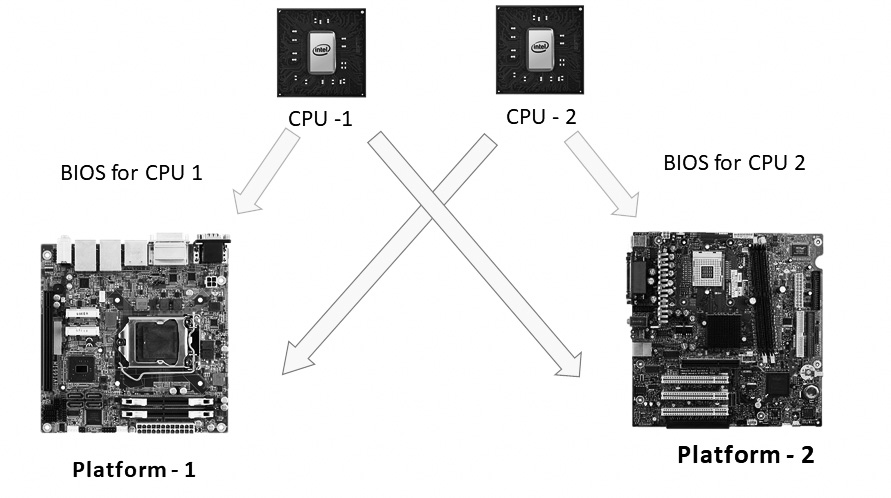
\includegraphics[width=0.7\linewidth]{design/cross-compatibility-design}
	\caption{Cross Compatibility Design}\label{fig:design-cross-compatibility-design}
\end{figure}

Figure \ref{fig:design-cross-compatibility-design} shows the general view of the Cross Compatibility of CPUs.

BIOS is the part of Integrated Firmware Image which resides at the End of the Binary table. The CPU swap can only occur in Specially designed Intel Designed Board only. Mainly because for each and every feature it required some hardware(H/W) requirements. If that H/W requirement not present. Then It will boot but doesn't support the Maximum speed.


\begin{figure}[h]
	\centering
	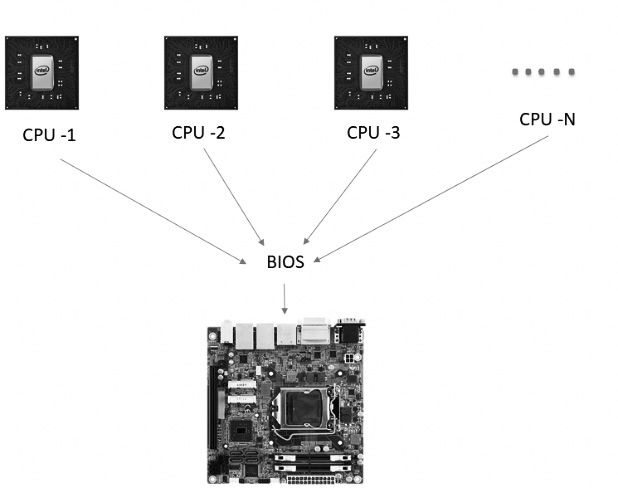
\includegraphics[width=0.7\linewidth]{design/bios-support-for-cross-compatibility}
	\caption{BIOS Support for Cross Compatibility}\label{fig:design-bios-support-for-cross-compatibility}
\end{figure}

Figure \ref{fig:design-bios-support-for-cross-compatibility} shows the BIOS role for identifying the CPUs during PEI phase.

As the number of Feature increases in the Silicon BIOS size also increases, usually the BIOS size varies from Platform to Platform and CPU to CPU., as we are integrating the Compatibility the BIOS size obviously increases. 

The structure of \gls{ifwi} is Shown in Figure \ref{fig:design-integrated-firmware-image}

\begin{figure}[h]
	\centering
	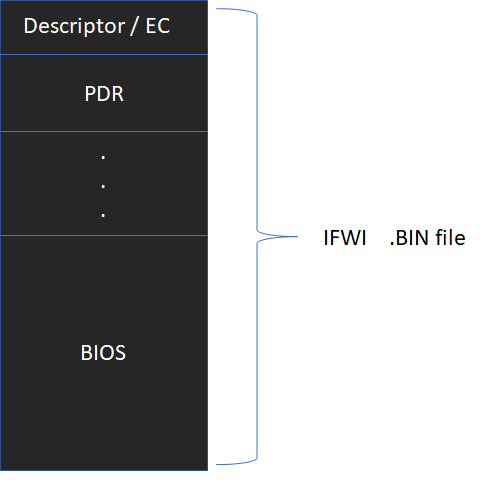
\includegraphics[width=0.7\linewidth]{design/integrated-firmware-image}
	\caption{Integrated Firmware Image}\label{fig:design-integrated-firmware-image}
\end{figure}


